%----------------------------------
% PARTIE 2 : Environnement technique
%----------------------------------

\section{Environnement technique}
\label{chp:part2:technical_environment}

L'intérêt de cette section est de décrire en amont les différents outils
techniques, matériels ou logiciels, qui ont dû être maîtrisés afin de mener à
bien les différentes missions qui m'ont été confiées.

\subsection{Matériel}
\label{chp:part2:subsct:hardware}

\subsubsection{STM32MP15 Wildcat}
\label{sec:wildcat_evalboard}

Le System on Chip ou SoC STM32MP15 présente sur une même puce  deux
microprocesseurs d’architecture ARM Cortex-A7 pouvant fonctionner jusqu'à une
fréquence de 800 MHz et un microcontrôleur ARM Cortex-M4 à 209 MHz. Ces trois
composants sont associés à une unité 3D GPU débouchant sur une interface
graphique MIPI-DSI et un convertisseur analogique numérique CAN.\\

Le processeur Cortex-A7 est un microprocesseur (ou MPU) performant très basse
consommation, doté d’une unité de gestion de mémoire (ou MMU), ce qui lui
permet de pouvoir exécuter un système d’exploitation. Pour le stage est
utilisé la distribution Linux open source de STMicroelectronics, OpenSTLinux,
avec le gestionnaire graphique Weston Wayland. \\

Le coprocesseur (ou MCU) Cortex-M4 est un microcontrôleur (donc dépourvu de
MMU) hautes performances et très basse consommation. Le coprocesseur est doté
d’une unité de traitement de signal (ou DSP). La présence du microcontrôleur
Cortex-M4 au sein du SoC permet de pouvoir déléguer une partie des tâches de
calculs à ce dernier, afin d’alléger la charge de travail du processeur
principal. STMicroelectronics promeut l’utilisation de l’environnement
STM32CubeMP1 pour le coprocesseur, par ailleurs, les capacités temps réel
rendent l’utilisation de RTOS ou RTEMS possible. \\

Ces deux processeurs possèdent un ensemble de périphériques qui peuvent être
soit propres à l’un des processeurs, soit partagés et donc avec la nécessité
d’être attribué à un processeur spécifique. L’attribution des périphériques
partagés s’effectue à travers le device tree, qui sera évoqué dans la partie
développement du projet. \\

\begin{figure}[H]
	\begin{center}
		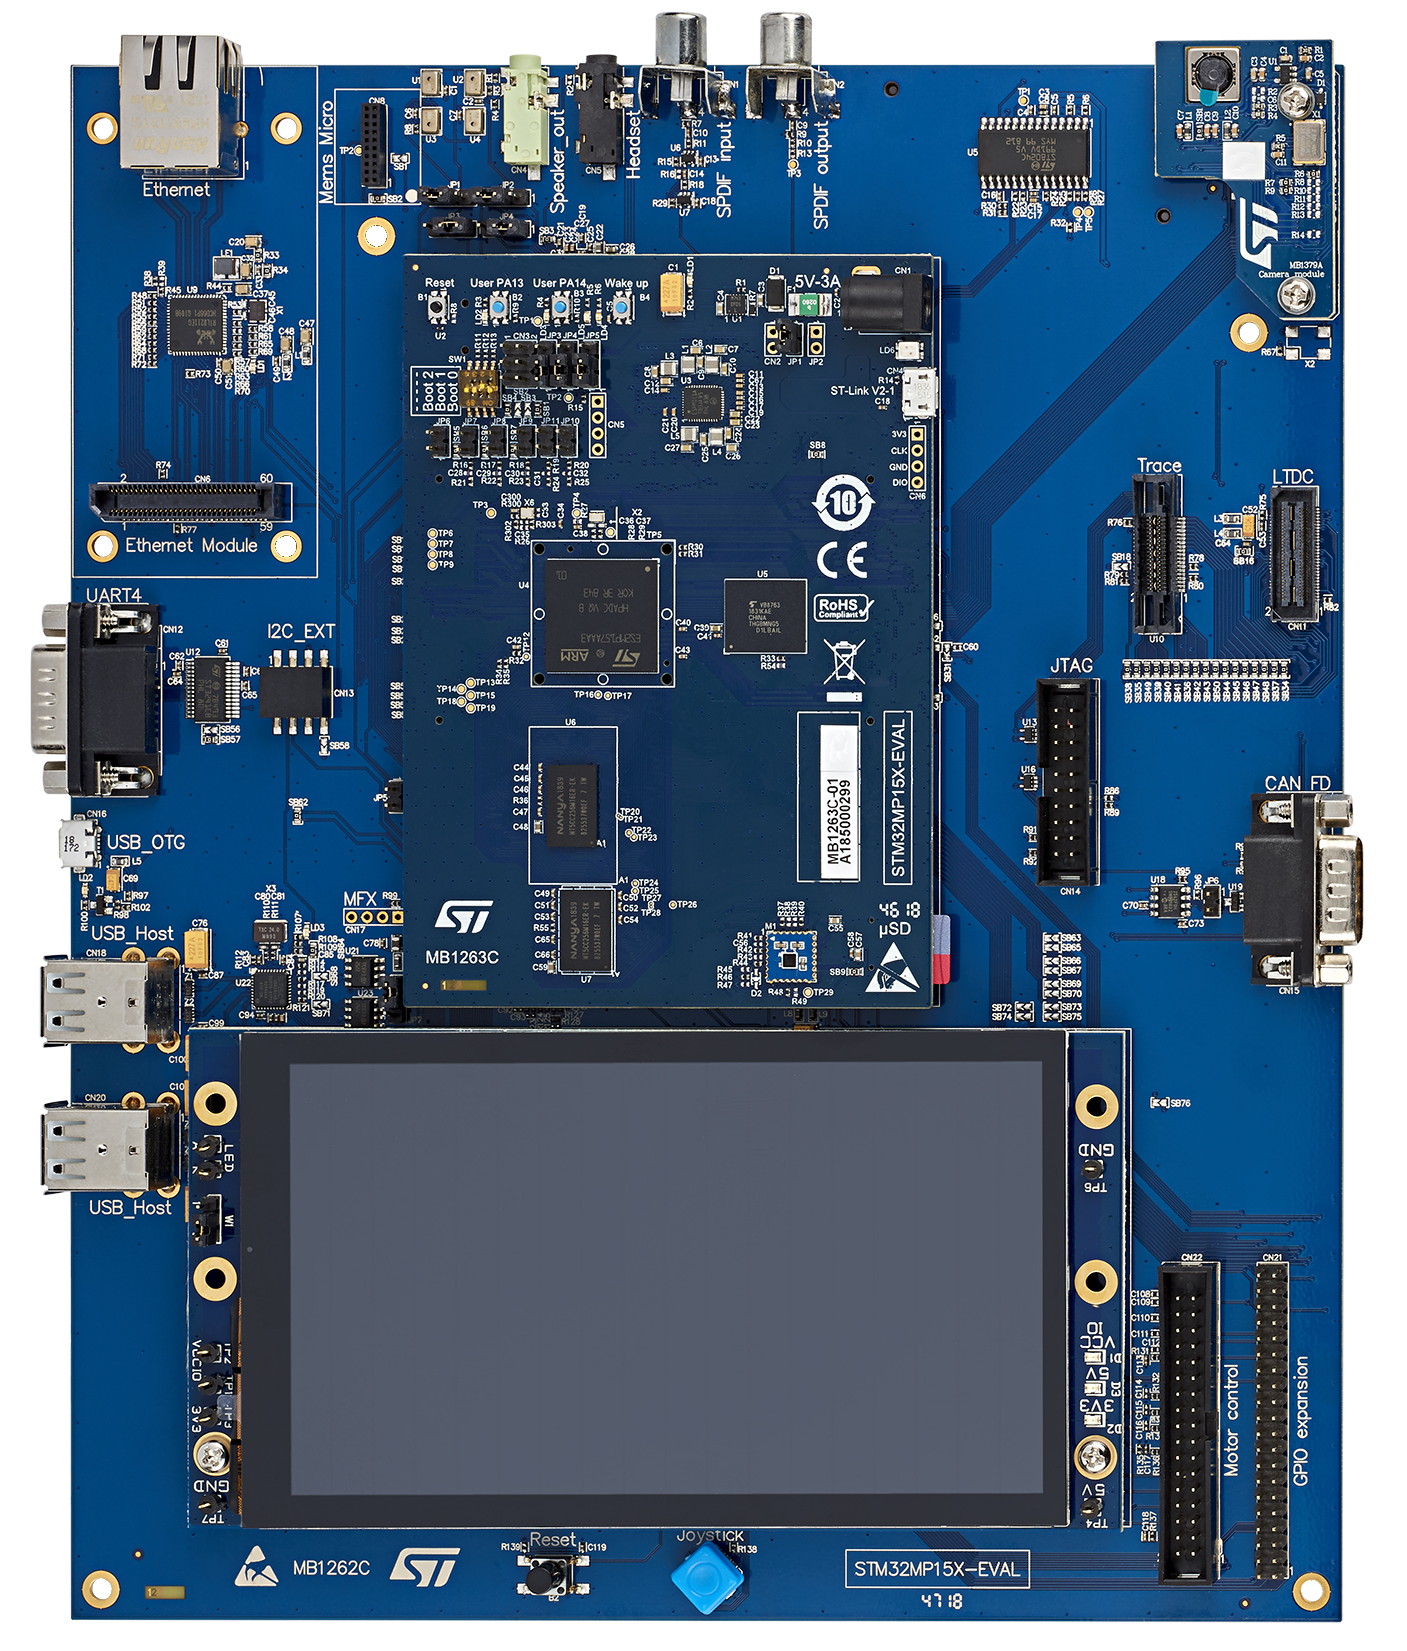
\includegraphics[scale=0.2]{\pathPartTwo/wildcat_evalboard}
		\caption{Carte référence STM32MP15 Evalboard}
	    \label{fig:wildcat_evalboard}
	\end{center}
\end{figure}

Le SoC STM32MP15 est interfacé sur la carte référence du SoC : la carte
STM32MP15 Evalboard. C'est une carte composite intégrant une carte mère sur
laquelle est soudée la puce, et une carte fille comprenant les différents
périphériques. D’un point de vue connectique, la carte comporte un connecteur
d'alimentation, un connecteur GPIO au standard Raspberry (broche de 2*20
pins), un autre utilisé spécifiquement pour le contrôle de moteur, un écran
tactile MIPI-DSI, 4 port USB-A, port micro USB On-The-Go (servant à faire
reconnaître la carte comme une clé USB), un convertisseur CAN accessible par
prise RS232, une prise RJ45 et deux prises audio jack 3.5mm. Le débogueur
embarqué ST-Link-V2 est accessible via le port UART 4 lui-même interfacé par
une prise USB-B micro. La carte contient également un port JTAG pour le
déboggage invasif. \\

Cette puce éléctronique se distingue grâce à sa connectique par ces nombreuses
fonctionnalités et augmente ainsi son champ d'application. Ses capacités et son
faible coût de revient sont également des atouts primordiaux de la puce sur le
marché.

\subsubsection{IPs CoreSight}
\label{sec:coresight_overview}

CoreSight est un nom déposé par ARM pour désigner une infrastructure de
composants électroniques permettant de tracer et déboguer des systèmes
basés sur des processeurs ARM. C'est par conséquent un nom générique pour tous
les composants ARM de traçage et débogage. \\

Les traces font référence à une quantité de données arbitraires fournissant
des informations du système à tout instant T. Ce sont ces traces, que l'on
analysera à posteriori et dont on parlera dans une section ultérieure (cf
partie \ref{sec:proper_decoding}). \\

Tout système Coresight est composé d'au moins d'un tableau de données stocké
dans une mémoire morte, appelée table ROM. Cette table en lecture seule est
accessible depuis un débogueur et fournit les adresses mémoires de tous les
composants Coresight implémentés. Dans cette table sont en réalité listés les
registres de base de chaque composant et le décalage des autres registres. En
connaissant cette adresse, en plus du décalage (ou offset) du registre que l'on
cherche à accéder, on obtient alors une cartographie de toutes les IPs ainsi
que leurs registres internes.  Le débogueur dispense ainsi d'un accès à tous
les éléments du système sans qu'il y ait un détail exhaustif de chaque
élément. \\

\begin{figure}[H]
	\begin{center}
		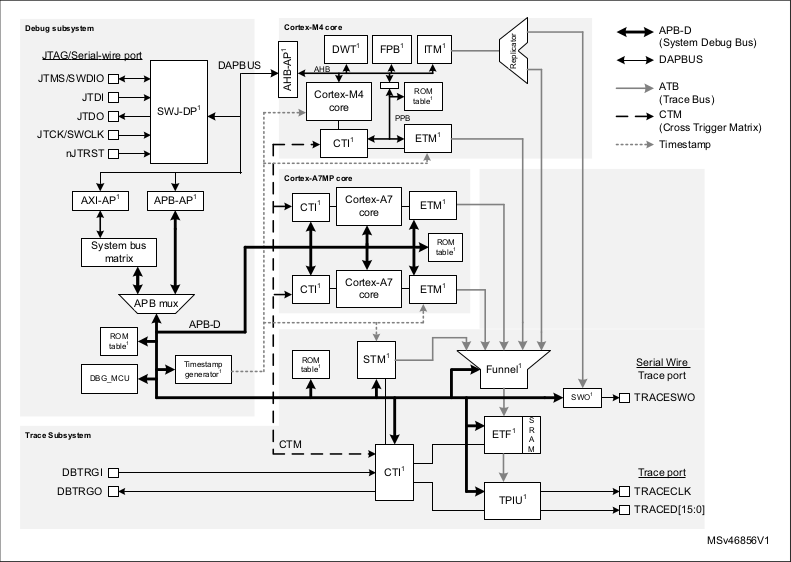
\includegraphics[width=\textwidth]{\pathPartTwo/debug_support_structure_diagram}
		\caption{Diagramme fonctionnel de l'infrastructure Coresight}
	    \label{fig:debug_support_structure_diagram}
	\end{center}
\end{figure}

Comme l'indique l'illustration \ref{fig:debug_support_structure_diagram}
ci-dessus, ce sous-système de composants s'articule autour des deux
processeurs Cortex-A7 et du coprocesseur Cortex-M4. On y observe de nombreux
composants dont certains directement impliqués dans la génération, le
transport et l'évacuation des traces Coresight. Ces derniers peuvent se
dissocier en trois catégories de composants : les sources, les puits et les
liens. \\

Les sources Coresight génèrent des données de traçage et de débogage. Ce sont
les premiers composants dans la chaîne d'acquisition de données. Dans le
système que l'on étudie, on s'attarde surtout sur les ETM (Embedded Trace
Macrocells).  Une relation de dépendance existe entre ces IPs et le processeur
sur lequel s'articule le système Coresight. Par exemple, les ETMv4 sont
spécifiques aux processeurs ARM Cortex-A8 tandis que les ETMv3 dans notre cas
s'appliquent à des Cortex-A7. De plus, selon la version de l'ETM, les capacités
diffèrent. Les ETMv1 et ETMv2, obsolètes versions des ETM, ne supportent pas
ce que les ETMv3 peuvent gérer. % Trop flou la dernière phrase 
Ces unités utilisent des bus de données de type AMBA (AHB et APB-D)
représentés sur la figure \ref{fig:debug_support_structure_diagram}. \\ 

Les liens sont des composants passifs qui peuvent s'apparenter à des
multiplexeurs et démultiplexeurs. Leur rôle est de diviser ou de multiplier
les flux de traces Coresight. Par exemple, le funnel (entonnoir en français)
est utilisé lorsqu'il y a plus d'une source génératrice. Il combine alors tous
ces flux en un seul pour aller vers un autre composant. \\

Les sinks (ou puits) permettent d'évacuer ou de stocker les traces véhiculées
au sein du système de débogage et sont les éléments finaux dans le système
Coresight. Dans le système étudié, on retrouve trois de ces IPs avec des
caractéristiques particulières. L'Embedded Trace Buffer, qui est un buffer
circulaire, fait l'acquisition des traces du système puis les stocke de
manière temporaire dans la SRAM (mémoire vive statique). Les deux autres
composants quant à eux évacuent les traces hors de la puce : le TPIU (Trace
Port Interface Unit) débouche sur le port JTAG de l'Evalboard, et le SWO
(Serial Wire Output) s'occupe d'une certaine trame, spécifique au
microcontrôleur Cortex-M4. Les deux derniers composants sont présents dans le
design hardware du système Coresight, mais restent malheureusement utilisables
en l'état. \\

Enfin, un élement central doit être mentionné puisqu'il coordonne le système.
Il s'agit du Timestamp Generator (Générateur de Timestamp). Dans un système où
plus d'un processeur est présent, il est possible que plusieurs instructions
assembleur soient exécutées quasiment en même temps par les CPUs. Dans le
résultat final il faut donc séquencer temporellement les étapes tracées. Le
timestamp generator (ou tsgen) autorise ceci en incrémentant un compteur et
envoyant à intervalles réguliers la valeur arbitraire de ce compteur. Ainsi
apparaissent dans le résultat final des trames indiquant le temps auquel les
trames se sont déroulées. Cela permet un retraçage temporel.

\subsection{Logiciel}
\label{chp:part2:subsec:software}

%\subsubsection{Environnement de développement et toolchain}
%\label{sec:env_toolchain}

%Dans une optique de praticité, les développeurs possèdent un ordinateur avec
%une distribution STUbuntu, un simple Ubuntu customisé par ST. Linux possède
%une facilité d'installation de programmes et d'outils permettant le
%développement kernel. Ainsi, une toolchain de cross-compilation est mise en
%place au lancement d'un terminal.
% what did I do in this paragraph ???

\subsubsection{GIT}
\label{sec:git}

Dans un projet d'envergure, avec une équipe de plus d'une dizaine de
personnes, il est nécessaire de hiérarchiser et d'organiser le travail et le
code source généré. Cela est possible avec GIT, un gestionnaire de version
open source et gratuit.

\subsubsection{OpenSTLinux}
\label{sec:openstlinux}

OpenSTLinux est la distribution Linux open source fournie par
STMicroelectronics pour aller sur les SoCs de type STM32MP15. C'est une
distribution basée sur Yocto, un projet facilitant la création d'outils et de
distributions Linux. Devenu un standard dans l'industrie IoT, Yocto intégre un
noyau OpenEmbedded. Le choix de ST à se tourner vers Linux, plutôt que de
créer son propre noyau fait bénéficier à l'entreprise les patchs et mises à
jour régulières faites par la communauté Linux, et permet ainsi d'avoir un
code très optimisé. 
% version avec laquelle j'ai travaillé ?

\subsubsection{Le noyau Linux}
\label{sec:linux_kernel}

\paragraph{Device tree}\mbox{}\\
\label{par:dt}

Le device tree est une arborescence de périphériques qui consiste en une
\textbf{description matérielle} de la carte électronique. Afin que le noyau
puisse effectuer des appels aux pilotes en fonction du matériel, il trouve
dans le device tree des structures de données des composants matériels tels
que les bus, périphériques, mémoires, horloges et CPU. \\

Sa finalité est donc de décrire les composants qui ne peuvent pas être
instanciés automatiquement lors du démarrage. À la différence d'une
architecture x86, ARM ne possède pas de bus avec "autodécouverte" des
composants et périphériques tel que le bus PCI. \\

Chaque fichier du device tree (.dts) est compilé individuellement par le dtc
(Device Tree Compiler) en Device Tree Blob (.dtb), mais la compilation globale
de tous les devices tree s'effectue par une règle dans le Makefile principal
du noyau : \textbf{make dtbs}. Ces devices tree blobs sont par la suite parsés et
interprétés lors de l'initilisation du noyau Linux.

\begin{figure}[H]
	\begin{center}
		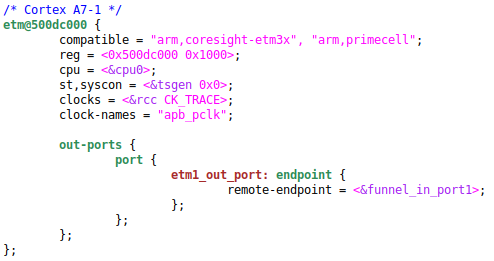
\includegraphics[scale=0.7]{\pathPartTwo/dts_etm}
		\caption{Exemple de structure du device tree d'un composant CoreSight}
	    \label{fig:dts_etm}
	\end{center}
\end{figure}

On retrouve le concept d'inclusion, à l'instar des entêtes C, donnant une
simple directive d'inclusion du contenu d'un fichier au sein d'un autre. On
retrouve ainsi des fichiers racines ".dtsi" correspondant à une description
commune entre plusieurs cartes électroniques inclus dans des device trees plus
spécifiques à chaque design. En pratique, ce fragment dtsi décrit
l'architecture interne du SoC (ici stm32MP151.dtsi). \\

Les adresses et offsets des composants sont définis dans une \textbf{memory
map} qui liste au format Excel tous les accès logiques des registres par des
bus de données. 

\paragraph{Kconfig}\mbox{}\\
\label{par:kconfig}

Au vu de la complexité du noyau Linux, de toutes les architectures existantes
ainsi que des divergences matérielles, la configuration des options du noyau
doit être simple et intuitive. Cela est rendu possible grâce à KConfig, une
interface de configuration des options du noyau. Dans chaque arborescence du
noyau, un fichier Kconfig définit les symboles et les define nécessaires à la
compilation de l'option. Pour une plus grande facilité de configuration, afin
d'éviter de passer du temps à tout configurer manuellement, une interface
utilisateur basée sur la librairie graphique NCurses est accessible avec la
commande : \textbf{make menuconfig}. Un arbre présentant toutes les options
disponibles s'affiche alors, et l'utilisateur peut choisir d'activer ou non
les options qu'il désire. En pratique, la compilation des pilotes Coresight,
primordiaux à l'utilisation du système, ne s'établie fait que si l'option est
activée à "yes".

\begin{figure}[H]
	\begin{center}
		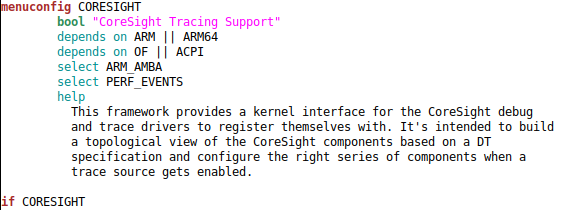
\includegraphics[scale=0.7]{\pathPartTwo/kconfig}
		\caption{Extrait de code du fichier Kconfig spécifique Coresight}
	    \label{fig:kconfig}
	\end{center}
\end{figure}

\subsubsection{Perf et le framework Coresight}
\label{sec:perf_coresight_framework}

Perf est un utilitaire Linux permettant la surveillance ainsi que le contrôle
d'évènements et la performance du noyau. Son nom est par ailleurs la
contraction du mot "performance". \\

Son code, intégré au noyau, se catégorise en deux sections : une partie espace
utilisateur qui fournit une API outil, la commande \textbf{perf} en tant que
telle, avec plusieurs sous-programmes utilitaires; et une seconde partie
espace noyau, qui gère les appels systèmes effectués dans l'espace utilisateur
et traite en conséquence les instructions reçues. \\

Cet utilitaire se base sur l'enregistrement d'évènements se déroulant à un
niveau matériel et logiciel. Cette supervision d'évènements lui confère en
conséquence la possibilité de mesurer des profils de performance avancés et de
contrôler des fonctions bas niveau. Il utilise notamment le PMU (Performance
Monitoring Unit). Ce composant, intégré dans tous les processeurs sophistiqués
produit aujourd'hui, surveille les micro évènements du CPU qu'il intègre comme
cela peut être le cas pour les cycles d'horloge écoulés, le nombre
d'instructions par cycle d'horloge ou encore le nombre de succès ou défauts de
cache. Cette PMU englobe 4 compteurs 32 bits, ainsi que des registres
spécifiques à sa configuration. \\

Chaque composant du système Coresight est instancié par des pilotes qui gèrent
séparément les IPs en elles-mêmes, mais aussi les différentes interfaces avec
leur environnement. Cela se traduit par des pilotes spécifiques pour
l'interface utilisateur sysfs ou bien des architectures pour l'intégration du
système Coresight avec l'outil perf (fichier coresight-etm-perf.c dans le
noyau). \\

Le framework et son intégration à l'outil perf rendent possible l'exploitation
dans l'espace utilisateur de profils de performance. Ces profils affichent
graphiquement ce que le processeur a exécuté. Dans le code source du noyau
Linux, les pilotes des composants sources (cf section
\ref{sec:coresight_overview}) font appel à une structure qui les modélisent en
tant que PMU. Le noyau de perf visualise ensuite cette abstraction
structurelle de la PMU lors du démarrage du noyau Linux comme le composant
utilisé. perf exerce ainsi un contrôle très précis sur l'activation et la
désactivation des traces. \\ 

\begin{figure}[H]
	\begin{center}
		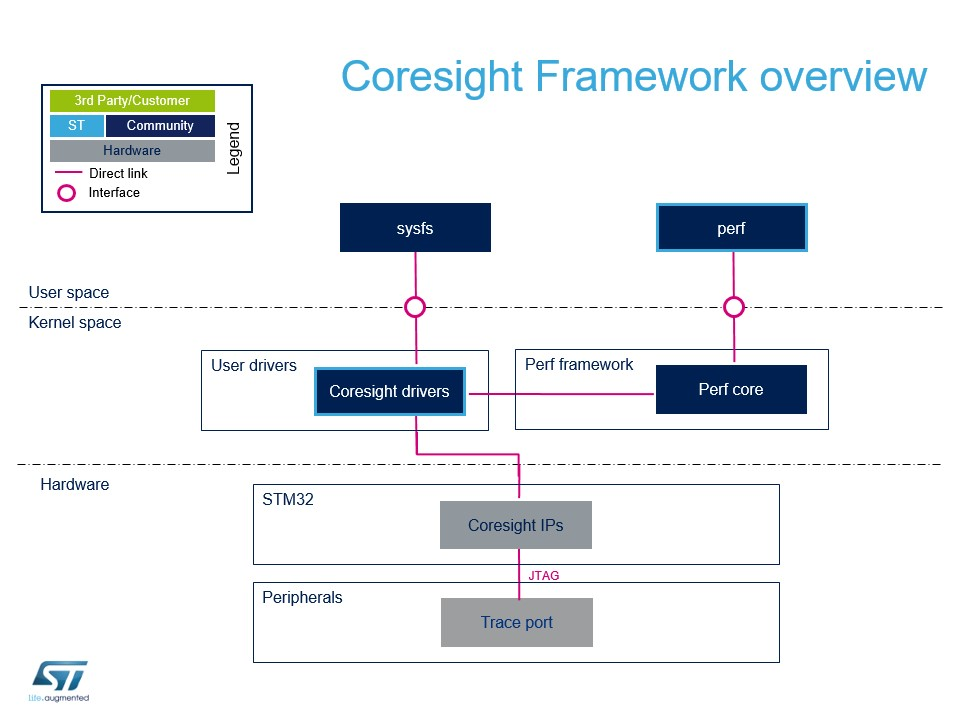
\includegraphics[width=\textwidth]{\pathPartOne/coresight_overview}
		\caption{Aperçu du framework Coresight et perf}
	    \label{fig:coresight_overview}
	\end{center}
\end{figure}
% https://01.org/linuxgraphics/gfx-docs/drm/trace/coresight/coresight.html
% search for 'coresight PMU'

%interface abstraite faisant
%l'intermédiaire entre les différents drivers PMU et le core de perf.
%cf. linaro blog from M. Poirier + Wildcat ref man
%
%
%https://unix.stackexchange.com/questions/326621/what-are-kernel-pmu-event-s-in-perf-events-list
%https://events.static.linuxfound.org/images/stories/pdf/lfcs2012_melo.pdf
%https://community.arm.com/developer/ip-products/processors/f/cortex-a-forum/5140/mrs-msr-banked-register
%https://www.kernel.org/doc/html/latest/trace/coresight/coresight.html
%https://qastack.fr/unix/326621/what-are-kernel-pmu-event-s-in-perf-events-list
%https://elinux.org/images/b/b3/Hardware_Assisted_Tracing_on_ARM.pdf
%http://rts.lab.asu.edu/web_438/project_final/Talk%209%20Performance%20Monitoring%20Unit.pdf
%https://fr.wikipedia.org/wiki/M%C3%A9moire_cache
